\message{ !name(zeta_ophiuchi.tex)}\documentclass[twocolumn,twocolappendix,trackchanges]{aastex63}
\usepackage{amsmath}
\newcommand{\code}[1]{\texttt{#1}}
\newcommand{\mesa}{\code{MESA}}
\newcommand{\MESA}{\code{MESA}}
\renewcommand{\labelitemii}{$\bullet$}
\newcommand{\kms}{{\mathrm{km\ s^{-1}}}}
\newcommand{\Msun}{{\mathrm{M}_\odot}}
\newcommand{\kev}{\mathrm{keV}}
\newcommand{\gk}{\ensuremath{\,\rm{GK}}}
\usepackage{CJK}
\DeclareRobustCommand{\Eqref}[1]{Eq.~\ref{#1}}
\DeclareRobustCommand{\Figref}[1]{Fig.~\ref{#1}}
\DeclareRobustCommand{\Tabref}[1]{Tab.~\ref{#1}}
\DeclareRobustCommand{\Secref}[1]{Sec.~\ref{#1}}
\newcommand{\zoph}{$\zeta$ Oph}

\newcommand{\todo}[1]{{\large $\blacksquare$~\textbf{\color{red}[#1]}}~$\blacksquare$}

\defcitealias{villamariz:05}{VH05}


\begin{document}

\message{ !name(zeta_ophiuchi.tex) !offset(1008) }
.

\todo{comment on rejuvenation and why braun\& langer did not find it}

\subsection{Variations in initial binary parameters}
\label{sec:bin_init}

The initial donor mass $M_1$, mass ratio $q=M_2/M_1$, and the period of the progenitor binary of \zoph\ cannot be directly
constrained from observations. We have explored variation in these values, and the
qualitative behavior of the models is similar.

Shorter initial periods results in larger post-RLOF orbital
velocities, and thus larger runaway velocities if the binary is
disrupted at the first SN (see \Secref{sec:SN_comp}). For example, taking $P$=75\,days
(cf.~100\,days in our fiducial model in \Secref{sec:best_model}), the
binary still experiences stable case B mass transfer, but the
post-RLOF orbital velocity of the accretor is about $60\,\kms$, that
is $\sim$$10\,\kms$ higher
than in our fiducial model.

Increasing the donor mass also has a similar effect on the post-RLOF orbital velocity of the accretor. Using
$M_1=30\,M_\odot$ (cf.
$25\,M_\odot$ in \Secref{sec:best_model}),
$M_2=17\,M_\odot$, and
$P$=100\,days, we obtain a post-RLOF velocity of
$65\,\kms$. However, this produces a stripped donor of
$\sim$16\,$M_\odot$ at RLOF detachment, with stronger wind mass loss. Therefore this binary is expected to widen relatively more than our fiducial model of \Secref{sec:best_model}, slowing down the secondary. The increased mass of the stripped star could also imply a lower chance of exploding for the donor, which might instead collapse to a black-hole instead (however, see \Secref{sec:SN_comp}).

The higher $M_1$ does not significantly change the post-RLOF total
mass of the accretor, with $M_2$ remaining about $\sim$20.5\,$M_\odot$, since
in our models accretion is regulated mostly by the spin up of the
accretor, and we do not couple the specific angular momentum of the transferred
material to the orbit or the donor's spin.

However, changing the initial mass ratio also changes the difference
between the main-sequence lifetime of the two stars, and thus how far
along the main sequence the accretor is at the onset of RLOF. The observed
position of \zoph\ on the HRD, particularly its relatively high
$T_\mathrm{eff}$ are difficult to reproduce assuming initially less
massive accretors (which would remain too cool even after accreting
mass), or more equal initial mass ratio (which would produce a too
evolved accretor at the onset of mass transfer).

\subsection{The explosion of the donor star}
\label{sec:SN_comp}

Throughout this study, we have assumed the ``binary SN scenario'' to
explain the runaway nature of \zoph:
after the mass transfer phase, the explosion of the donor disrupts the
binary and ejects the accretor at roughly its pre-explosion orbital
velocity \citep[e.g.,][]{renzo:19walk}. This fate occurs to the
majority of massive binary systems, and \zoph\ might be the best
example of it \citep[e.g.,][]{blaauw:52, blaauw:61,
  hoogerwerf:00}. \cite{neuhauser:20} suggested not only the companion
successfully exploded producing the pulsar PSR B1706-16, but that the
explosion produced radioactive $^{60}\mathrm{Fe}$ which polluted
Earth.

From kinematic and orbital considerations they estimated the pulsar
received a natal kick of
$253\pm54\,\kms$, which would be sufficiently large to unbind the binary \citep{kalogera:96, tauris:15}.  The ejecta mass would depend on the post-RLOF wind mass loss of our donor star, which we do not model.  At the end of our binary model (black diamond in \Figref{fig:HRD_both}), our stripped donor is
$\sim$$9.4\,M_\odot$, with a surface H fraction of $X\lesssim0.2$ for
a layer of $\Delta M \simeq 2.5\,M_\odot$.  Its wind mass-loss rate is
$\sim10^{-5}\,M_\odot \ \mathrm{yr^{-1}}$ (cf.~\Figref{fig:MT}),
likely to increase as it contracts into a Wolf-Rayet star and
increases its luminosity and effective temperature. We expect its
explosion to appear as H-less type Ib SN. Although our stripped donor
is rather massive, recent studies hints at a higher ``explodability''
of donor stars in binary systems \citep[e.g.,][]{schneider:21,
  laplace:21, vartanyan:21}.

We have neglected the impact of the explosion on the structure of the
accretor star. At the time of the explosion, the accretor subtends a
solid angle $\sim$$R^2/a^2\simeq
2\times10^{-3}$\,steradians with $R$ the accretor radius and
$a$ the binary separation. We neglect the post-RLOF wind-driven orbital widening for this estimate.  The blast wave will hit the accretor causing mass loss -- directly via ablation and by injecting energy in the envelope, inflating it and enhancing its wind \citep{wheeler:75, tauris:98, podsiadlowski:03, hirai:18}.  Because of the SN shock, the just ejected new runaway star might appear bloated and redder (long before it overtakes the slowing SN remnant). The impact of this brief out of thermal equilibrium phase on the stellar spin should be investigated further.

Using 2D hydrodynamic simulations of the star-SN ejecta interactions in close binaries ($a\lesssim
60\,R_\odot$, cf. $a\gtrsim
343\,R_\odot$ in our fiducial binary model), \cite{hirai:18} found that the companion star recovers its pre-explosion luminosity and effective temperature within a few years to decades, and the amount of mass removed by the SN shock is
$\lesssim10^{-2}\,M_\odot$.  The SN ejecta might also pollute the surface of the runaway depositing processed nuclear material \citep[e.g.,][]{przybilla:08, suda:21}. However, for the large final separation of our model, little pollution is expected and enhahnced mass loss and inward mixing might quickly dilute any signature below detectable levels.


\section{Conclusions}
\label{sec:conclusions}

We presented self-consistent spherically-symmetric \texttt{MESA}
calculations of a binary system where both stars are evolved
simultaneously and coupled. As a first application, we focused on
finding a model for \zoph, assuming its runaway nature is explained by
the binary SN scenario.

We found that it is possible to explain the observed features of
\zoph\ with a relatively wide and massive binary initialized with
$M_1=25\,M_\odot$, $M_2=17\,M_\odot$, and $P=100$\,days at metallicity
$Z=0.01$ (see \Secref{sec:best_model}). This binary system experiences dynamically-stable Roche
lobe overflow after the end of the main sequence of the initially more massive star
(case B). Standard stellar physics assumptions for modeling rotation,
mixing, and mass transfer in binaries (see \Secref{sec:methods} and
Appendix~\ref{sec:software}) reproduce reasonably well the
main features of \zoph. Specifically,
$\sim$$1.5-2$\,Myrs after the end of mass transfer, corresponding to the
remaining donor's lifetime at the end of our simulations plus the kinematic age of \zoph,
the accretor star in our model has the following quantities in the correct ballpark:
\begin{itemize}
\item Luminosity and effective temperature;
\item Total mass;
\item Runaway space velocity;
\item Fast surface rotation (albeit possibly on the low side, cf.~weak wind problem);
\item enhanced $^4\mathrm{He}$ and $^{14}\mathrm{N}$ surface mass fraction;
\item small variations in $^{12}\mathrm{C}$ and $^{16}\mathrm{O}$ surface mass fractions.
\end{itemize}

We emphasize that the surface composition alone would not be a smoking-gun,
especially given the large uncertainties in the treatment of rotation
and mixing in stellar evolution models. However, alternative scenarios where \zoph\
evolved as a single fast-rotating star require ad-hoc explanations for the runaway velocity,
and have been shown by \citetalias{villamariz:05} to struggle in reproducing
surface mass fractions, apparent age, mass, and rotation rate simultaneously.

In contrast with \cite{vanrensbergen:96}, in our model the
$^{14}\mathrm{N}$- and $^4\mathrm{He}$-rich surface composition is not
the result of pure outward rotational mixing.  Instead, this material
is transferred from the receeding core of the donor star and mixed
from the surface inwards by rotation and, to a smaller degree, by
thermohaline mixing.  Thus, the present day surface mass fractions of
\zoph\ put a coupled constrain the mass transfer efficiency and mixing
in the accretor. Therefore, such star should \emph{not} be used to
calibrate models of rotational mixing in single star evolution, nor
its more extreme version of chemically homogeneous evolution.

The spin up of the accreting star occurs late in its evolution
($t\gtrsim7.25$\,Myr for our fiducial binary) and
reaches to critical surface rotation
$\omega/\omega_\mathrm{crit}\simeq 1$. % This allows the accretor star
% to be simultaneously nitrogen rich and still fast rotating after the
% mass transfer phase.
The treatment of close-to-critical rotation
impacts the accretion efficiency, the radius evolution, and the inward
mixing.

An important difference we find between our accretor model and
comparable fast-rotating single star models is their internal rotation
profile. Single-stars rotating rapidly from birth are initialized as
rigid rotators, and spin down significantly both at the surface and
inside. Conversely, in our accretor models angular momentum is
injected late and from the top. When this angular momentum is
transported into the core by the Spruit-Tayler dynamo, it results in a
much faster rotating helium core, with potential implications for the
final explosion and the resulting compact object born from the
accretor star in an interacting binary system. %  We emphasize that our models assume a
% Spruit-Tayler dynamo \citep{spruit:02} for the transport of angular
% momentum. Recently, \cite{fuller:19} proposed a stronger angular
% momentum transport which would presumably result in a faster spin down
% of the surface (possibly allowing for more accretion during mass
% transfer) and even more significant core spin-up in our accretor.


We also consider variations in the initial parameters and in the
implementation of physical processes, discussed in
\Secref{sec:discussion}.  Less massive accretors remain too cool
throughout the evolution to be compatible with \zoph, and more equal
initial mass ratios lead to a more evolved accretor at the onset of
mass-transfer, again resulting in too cool temperatures. Increasing
the donor's initial mass might result in stripped stars unlikely to
form a neutron star in their final SN explosion.

Improving our understanding of the evolution of the initially less
massive stars in massive binary systems is crucial for the upcoming
large surveys (astrometric, photometric, spectroscopic, and in time domain) and for the understanding of the evolution of
gravitational-wave progenitors in isolated binaries. Although
presently single, the nearest O-type star to Earth, \zoph, can be used
as an anchor point for the modeling of accretors. Our models
demonstrate that a broad agreement with observations can be
achieved with standard stellar evolution assumptions. Future efforts
should extend these models to a wider mass, period, mass ratio, and metallicity
range to investigate the impact of binary evolution on the life,
explosion, and after-life of the secondary stars in massive binary
systems.

\software{
  \MESA\ \citep{paxton:11,paxton:13,paxton:15,paxton:18,paxton:19},
  \texttt{mesaSDK} \citep{mesasdk},
  \texttt{ipython/jupyter} \citep{ipython},
  \texttt{matplotlib} \citep{matplotlib},
  \texttt{mesaPlot} \citep{mesaplot},
  \texttt{NumPy} \citep{numpy}.
}

\acknowledgements{We are grateful to E.~Zapartas, A.~Jermyn,
  M.~Cantiello, and R.~Neuh\"auser for helpful discussions.}

\appendix

\section{\texttt{MESA} setup}
\label{sec:software}

We use \code{MESA} version 15140 to compute our models.  The
\code{MESA} equation of state (EOS) is a blend of the OPAL \citet{Rogers2002}, SCVH
\citet{Saumon1995}, PTEH \citet{Pols1995}, HELM \citet{Timmes2000},
and PC \citet{Potekhin2010} EOSes.

OPAL \citep{Iglesias1993, Iglesias1996} provides the main radiative
opacities, with low-temperature data from \citet{Ferguson2005} and the
high-temperature from \citet{Buchler1976}. Electron conduction
opacities are from \citet{Cassisi2007}.

Nuclear reaction rates are a combination of rates from NACRE
\citep{Angulo1999}, JINA REACLIB \citep{Cyburt2010}, plus additional
tabulated weak reaction rates \citet{Fuller1985, Oda1994,
  Langanke2000}. Screening is included via the prescription of
\citet{Chugunov2007}.  Thermal neutrino loss rates are from
\citet{Itoh1996}. We use a
22-isotope nuclear network (\texttt{approx\_21\_plus\_cr56}).

The inlists, processing scripts, and model output will be made available at~\url{10.5281/zenodo.4701565}.

\section{Resolution tests}
\label{sec:res_tests}


\begin{figure*}[hp]
  \centering
  \includegraphics[width=\textwidth]{spatial_res_plot}
  \caption{Left: HRD comparison for our fiducial binary model varying
  the number of mesh points. We only show the evolution until our definition
  of RLOF detachment. Right: number of mesh points as a
  function of timestep number. In both panels, the blue/cyan tracks show the donor stars, the
red/pink tracks show the accretor. Thicker dashed lines correspond to
the models at higher resolution (i.e., lower $\Delta$ which indicates
the value of \texttt{mesh\_delta\_coeff}).}
\label{fig:sp_test}
\end{figure*}



We extensively check the numerical convergence of our stellar
evolution calculations with increasing number of mesh
points. \Figref{fig:sp_test} shows that all the features described
extensively here do not vary when increasing the spatial resolution by
decreasing \texttt{mesh\_delta\_coeff}. The right panel shows the
number of mesh points for the accretor (top) and donor (bottom) as a
function of the model number (akin to an arbitrary time
coordinate). About $\sim$7000 \texttt{MESA} models are used to compute
the binary evolution. The higher resolution run has $\sim 20\%$ more
mesh points. The left panel shows the HRD evolution until the
detachment of the binary for the two accretor models (pink/red) and
the two donor models (blue/cyan).

Similarly, we tested the numerical convergence with decreasing
timestep size. This can be done decreasing the parameter
\texttt{mesh\_time\_coeff}. However, we were unable to successfully
compute models at higher temporal resolution. Partial results show a
good agreement with our fiducial model until \texttt{MESA} becomes
unable to find a satisfying numerical solution to the stellar
structure equations (typically
during RLOF). Lower temporal resolution models showed a similar
qualitative agreement but increased noisiness during the late RLOF
phase. For our fiducial model the adaptive timestep size never exceeds
$10^{3.8}$\,years with typical pre-RLOF timesteps of the order of $10^{3.2}$\,years
and sub-decade during RLOF. The main factor limiting the timestep
sizes is the change of surface angular momentum in both stars during
the mass transfer.


\section{Internal composition profile evolution}
\label{sec:X_fig}


\Figref{fig:composition_huge} compares the internal evolution of the composition
profile of single rotating stars with our accretor model.
We show mass fractions of $^{12}\mathrm{C}$  and $^{16}\mathrm{O}$ to complement the
mass fraction of $^{14}\mathrm{N}$ shown in \Figref{fig:n14}, and
reproduced also in the middle panel of \Figref{fig:composition_huge}.


\begin{figure*}[hp]
  \centering
  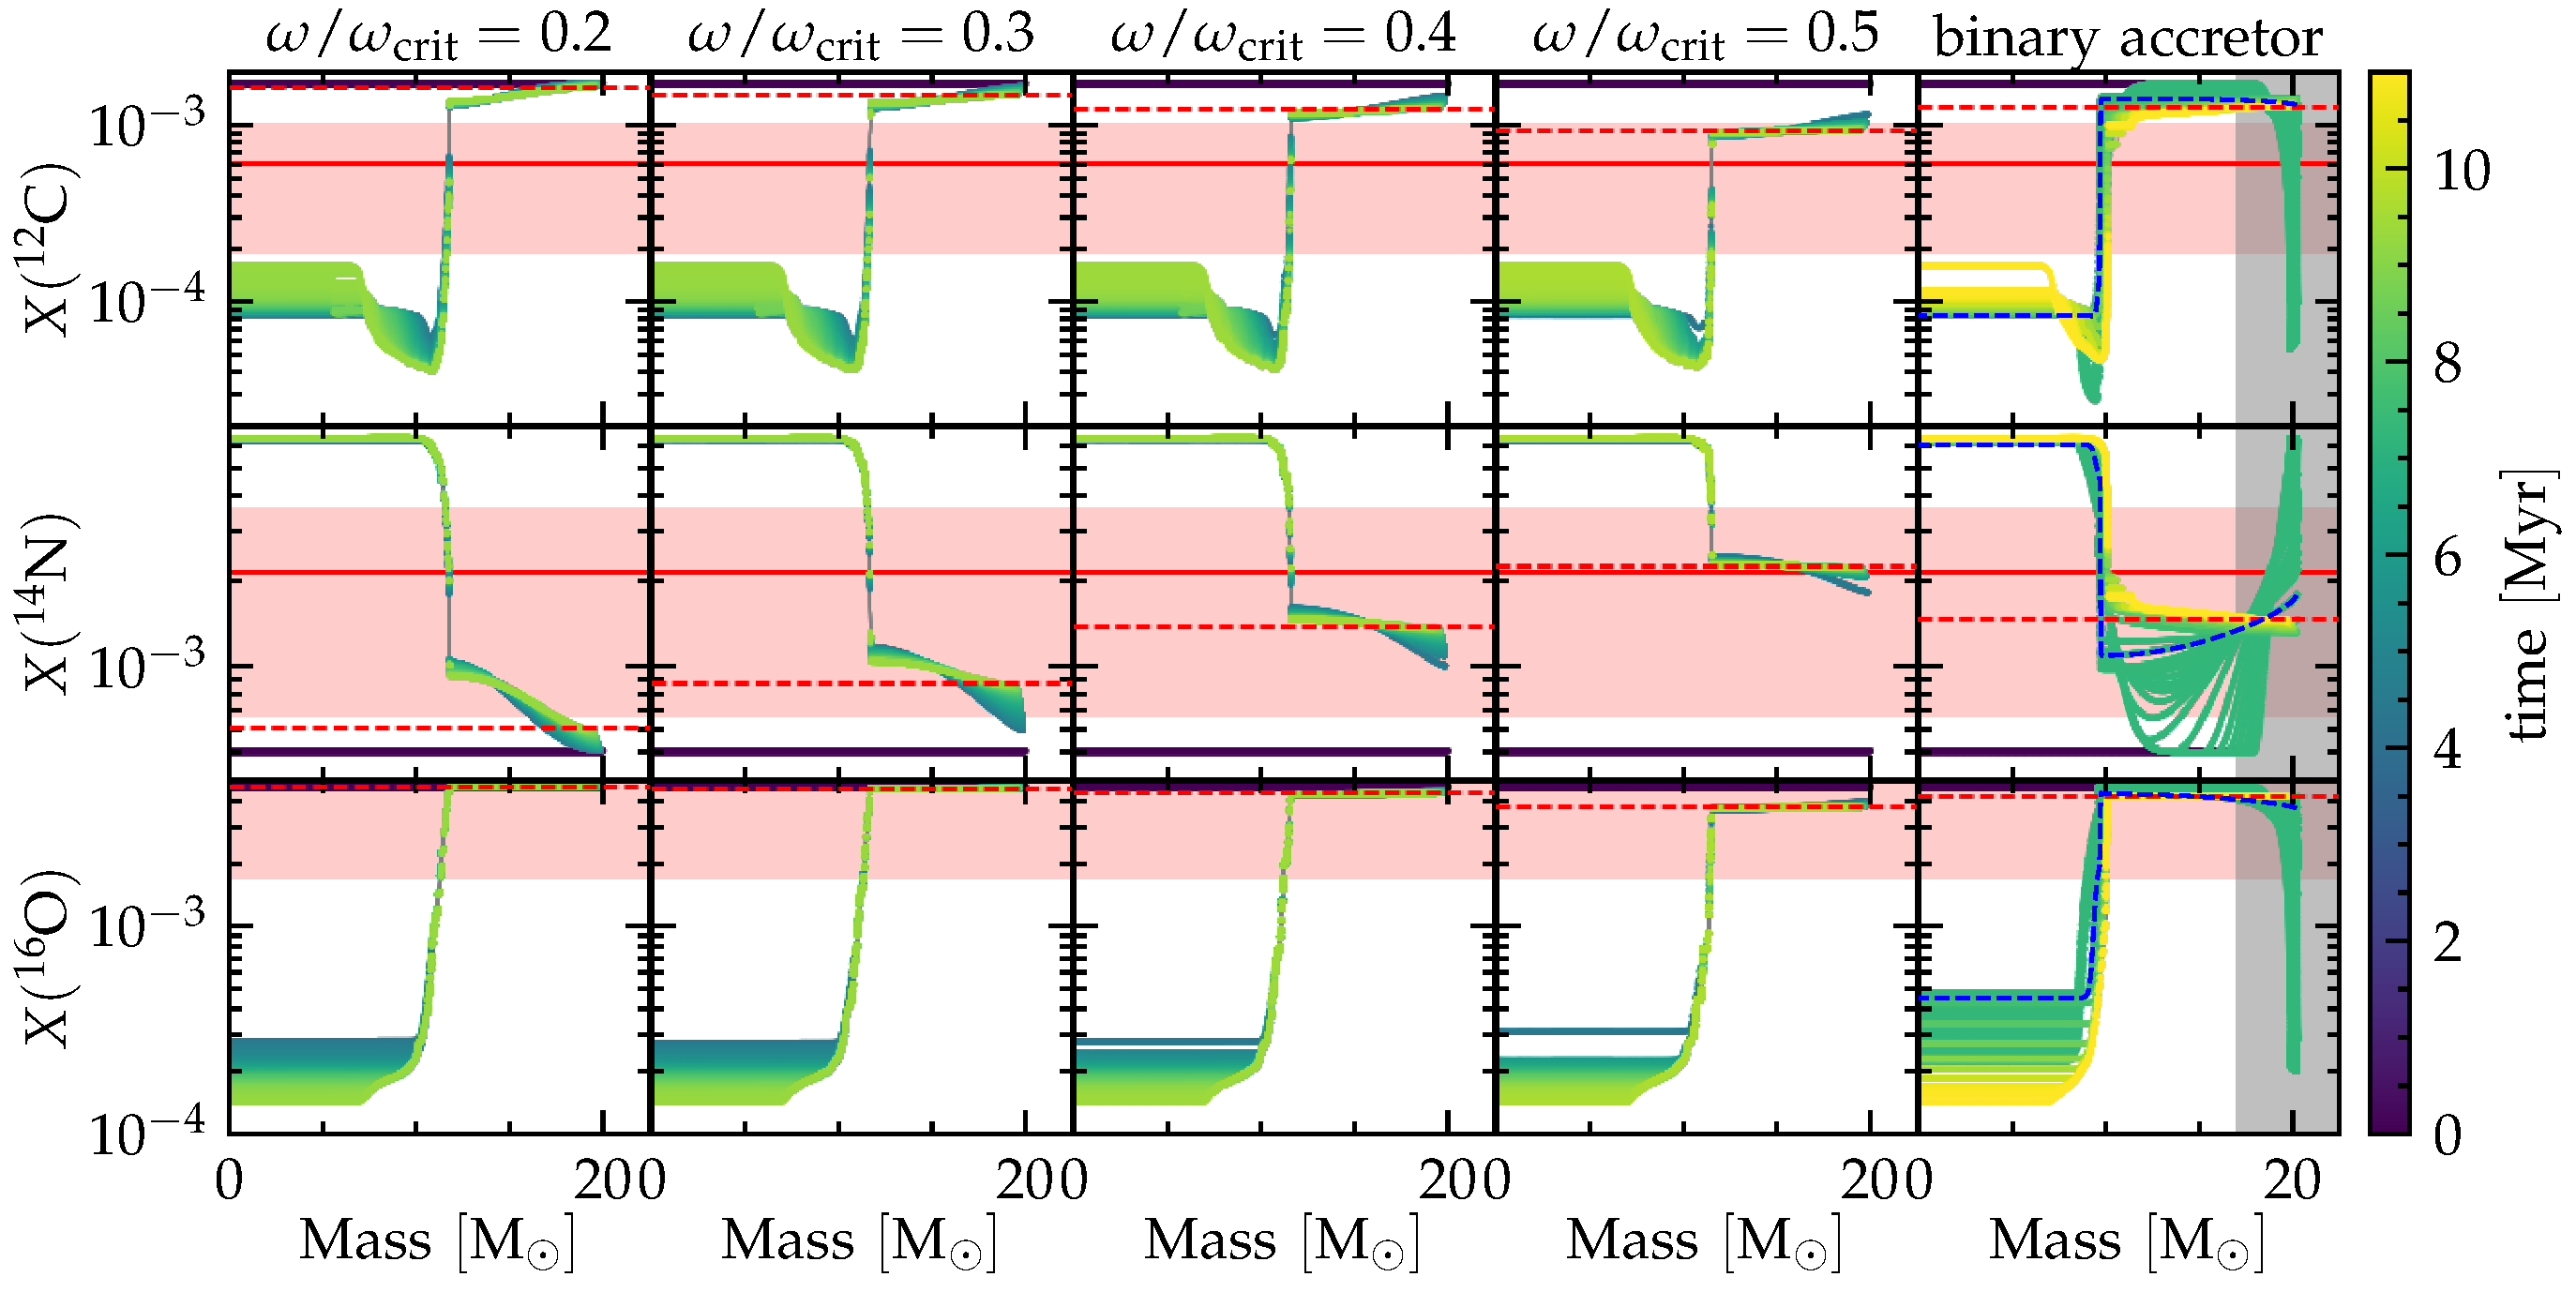
\includegraphics[width=\textwidth]{huge_composition}
  \caption{Same as \Figref{fig:n14}, but for $^{12}\mathrm{C}$ (top
    panel), and $^{16}\mathrm{O}$ (bottom panel). The first four
    panels show single rotating stars of initially $20\,M_\odot$, the
    rightmost panel shows the accretor in our fiducial binary. The middle panel is
    exactly the same as \Figref{fig:n14}. Thick red dotted lines mark the
    initial mass fractions, thin red dashed lines the TAMS surface mass
    fraction, the solid red lines and the semi-transparent red bands
    correspond to the values inferred by \citetalias{villamariz:05}
    using the surface H mass fraction from our model. The tracks go
    from dark (roughly corresponding to ZAMS) to light colors, with the
    lightest color corresponds to TAMS.}
  \label{fig:composition_huge}
\end{figure*}

\message{ !name(zeta_ophiuchi.tex) !offset(1009) }

\end{document}

%%% Local Variables:
%%% mode: latex
%%% TeX-master: t
%%% End:
